% !TEX root = ../chem_ia.tex
\begin{figure}[h!]
     \centering
     \begin{subfigure}[t]{0.45\textwidth}
         \centering
         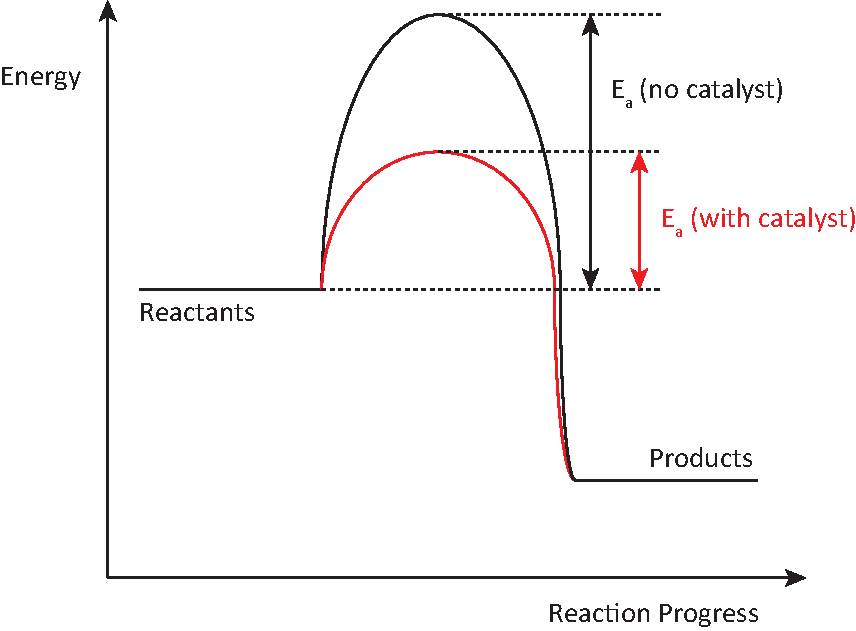
\includegraphics[width=\textwidth]{fig/images/catalyst_enthalpy.pdf}
         \caption{The catalyst provides an alternative pathway for the reaction with a lower $E_a$}
         \label{fig:catalyst-enthalpy}
     \end{subfigure}
        \hfill
     \begin{subfigure}[t]{0.45\textwidth}
         \centering
         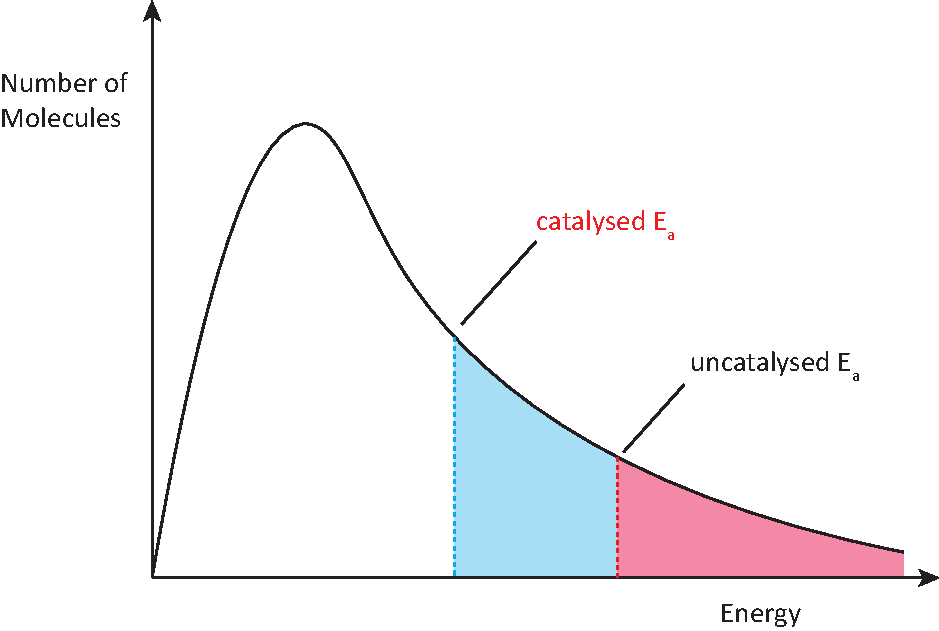
\includegraphics[width=\textwidth]{fig/images/catalyst_maxwell.pdf}
         \caption{The Maxwell Boltzmann Distribution shows how more molecules can then react as a larger proportion of molecules have sufficient energy ($>E_a$).}
         \label{fig:catalyst-maxwell}
     \end{subfigure}
    \caption{Catalyst Function}
    \label{fig:background_1}
\end{figure}